\documentclass[10pt,a4paper]{article}

% -- math packages --
\usepackage{amsmath}
\usepackage{amsfonts}
\usepackage{amssymb}
\usepackage{amsthm}
\usepackage{mathrsfs}

% -- utils --
\usepackage{ifthen}

% -- layout packages --
\usepackage{multicol}
\usepackage{fancyhdr}
\usepackage[margin = 1.2cm, includeheadfoot]{geometry}
\addtolength{\textheight}{1cm}
\addtolength{\footskip}{-1cm}
\usepackage{tcolorbox}
\usepackage{xcolor}
\usepackage{colortbl}

% -- language and encoding packages --
\usepackage[ngerman]{babel}
\usepackage[utf8]{inputenc}
\usepackage[T1]{fontenc}

% -- header definition --
\pagestyle{fancy}
\fancyhf{}
\fancyhead[R]{Seite \thepage}
\fancyhead[L]{Analysis Zusammenfassung}
\fancyhead[C]{Nicolas Trüssel}

% -- titlepage setup --
\author{Nicolas Trüssel}
\title{Analysis Zusammenfassung}

% -- multicols setup --
\setlength{\columnseprule}{0pt}
\setlength{\columnsep}{4mm}

% -- theorem environments --
\tcbset{before=, after=, top=2mm, bottom = 2mm, left=2mm, right=2mm, title=, arc=0mm, colframe=gray, boxrule=0.5pt}

\colorlet{mathyellow}{yellow!10}
\colorlet{mathorange}{orange!10}
\colorlet{mathred}{red!10}
\colorlet{mathpurple}{blue!10}
\colorlet{mathblue}{cyan!10}
\colorlet{mathgreen}{green!10}

\theoremstyle{plain}
\newtheorem{math_definition}{Definition}[section]
\newenvironment{definition}[1][]
	{\begin{tcolorbox}[colback=mathyellow]\begin{math_definition}
		\ifthenelse{ \equal{#1} {} }
			{}
			{\highlight{(#1)}}
	}
	{\end{math_definition}\end{tcolorbox}}
	
\newtheorem{math_proofhelp}{Beweishilfe}[section]
\newenvironment{proofhelp}[1][]
	{\begin{tcolorbox}[colback=mathgreen]\begin{math_proofhelp}
		\ifthenelse{ \equal{#1} {} }
			{}
			{\highlight{(#1)}}
	}
	{\end{math_proofhelp}\end{tcolorbox}}

\newtheorem{math_hint}{Trick}[section]
\newenvironment{hint}[1][]
	{\begin{tcolorbox}[colback=mathgreen]\begin{math_hint}
		\ifthenelse{ \equal{#1} {} }
			{}
			{\highlight{(#1)}}
	}
	{\end{math_hint}\end{tcolorbox}}

\newtheorem{math_shortcut}{Shortcut}[section]
\newenvironment{shortcut}[1][]
	{\begin{tcolorbox}[colback=mathgreen]\begin{math_shortcut}
		\ifthenelse{ \equal{#1} {} }
			{}
			{\highlight{(#1)}}
	}
	{\end{math_shortcut}\end{tcolorbox}}

\theoremstyle{definition}
\newtheorem{math_theorem}{Theorem}[section]
\newenvironment{theorem}[1][]
	{\begin{tcolorbox}[colback=mathred]\begin{math_theorem}
		\ifthenelse{ \equal{#1} {} }
			{}
			{\highlight{(#1)}}
	}
	{\end{math_theorem}\end{tcolorbox}}
	
\newtheorem{math_corollary}[math_theorem]{Korallar}
\newenvironment{corollary}[1][]
	{\begin{tcolorbox}[colback=mathorange]\begin{math_corollary}
		\ifthenelse{ \equal{#1} {} }
			{}
			{\highlight{(#1)}}
	}
	{\end{math_corollary}\end{tcolorbox}}

	
% -- custom commands - text --
\newcommand{\highlight}[1]{\textbf{\textup{#1}}}

% -- custom commands - table --
\newcommand{\fracsize}{\rule[-2ex]{0pt}{5ex}}
\newcolumntype{C}[1]{>{\fracsize\centering\arraybackslash$}m{#1}<{$}}
	
% -- custom commands - math --
\newcommand{\abs}[1]{\left\vert #1 \right\vert}
\newcommand{\norm}[1]{\left\Vert #1 \right\Vert}
\newcommand{\dotp}[2]{\left\langle #1, #2 \right\rangle}
\newcommand{\emath}{\boldsymbol{e}}
\renewcommand{\imath}{\boldsymbol{i}}
\newcommand{\Image}{\mathrm{Im}}
\renewcommand{\d}{\mathrm{d}}
\newcommand{\diff}[3][]
	{\frac{
		\ifthenelse{\equal{#1} {}} {\d #2} {\d^{#1} #2}
	}{
		\ifthenelse{\equal{#1} {}} {\d #3} {\d #3^{#1}}
	}
}
\newcommand{\pdiff}[3][]
	{\frac{
		\ifthenelse{\equal{#1} {}} {\partial #2} {\partial^{#1} #2}
	}{
		\ifthenelse{\equal{#1} {}} {\partial #3} {\partial #3^{#1}}
	}
}
\newcommand{\range}[2]{\Bigg\vert_{#1}^{#2}}
\renewcommand{\div}{\mathrm{div}}

\DeclareMathOperator{\arsinh}{arsinh}
\DeclareMathOperator{\arcosh}{arcosh}
\DeclareMathOperator{\artanh}{artanh}
\DeclareMathOperator{\arcoth}{arcoth}

\DeclareMathOperator{\Rot}{Rot}


\begin{document}
\setlength{\parindent}{0em} 
\let\clearpage\relax

%% !TeX root = ../Main.tex
\section{Logik und Grundlagen}
	\subsection{Funktionen}
		\begin{definition}
			Sei $f: X \to Y$ eine Abbildung.
			\begin{enumerate}
				\item f heisst \highlight{surjektiv}, falls $\forall y \in Y \, \exists x \in X \, : \, f(x) = y$
				\item f heisst \highlight{injektiv}, falls $\forall x_1, x_2 \in X \, : \, f(x_1) = f(x_2) \Rightarrow x_1 = x_2$
				\item f heisst \highlight{bijektiv}, falls f injektiv und surjektiv ist.
			\end{enumerate}
		\end{definition}
% !TeX root = ../Main.tex
\section{Zahlen und Vektoren}
	\begin{multicols}{2}
			\begin{definition}[Eigenschaften der Norm]\hfill\\
				Eine Norm hat folgende Eigenschaften:
				\begin{enumerate}
					\item Definitheit: $\norm{x} \geq 0, \quad \norm{x} = 0 \Rightarrow x = 0$
					\item Positive Homogenität: $\norm{\alpha x} = \abs{\alpha} \norm{x}$
					\item Dreiecksungleichung: $\norm{x + y} \leq \norm{x} + \norm{y}$
				\end{enumerate}
			\end{definition}
			\begin{theorem}[Archimedisches Prinzip]
				Zu jeder Zahl $0 < b \in \mathbb{R}$ gibt es ein $n \in \mathbb{N}$ mit $b < n$
			\end{theorem}
			\begin{theorem}[Young Ungleichung]
				Für $x,y \in \mathbb{R}, \varepsilon > 0$ gilt
				\begin{equation*}
					2 \abs{x \cdot y} \leq \varepsilon x^2 + \frac{1}{\varepsilon} y^2
				\end{equation*}
			\end{theorem}
			\begin{theorem}[Dreiecksungleichungen]
				Es gilt: 
				\begin{align*}
					\abs{\sum\limits_{i=1}^{n} x_i} &\leq \sum\limits_{i=1}^{n} \abs{x_i} \\
					\abs{\prod\limits_{i=1}^{n} x_i} &= \prod\limits_{i=1}^{n} \abs{x_i} \\
					\abs{x \pm y} &\geq \abs{\abs{x} - \abs{y}} 
				\end{align*}
			\end{theorem}
%		\subsection{Supremum und Infimum}
%			\begin{definition}
%				Eine Menge $A \subset \mathrm{R}$ heisst \highlight{nach oben beschränkt}, falls gilt
%				$$
%					\exists b \in \mathrm{R} \, \forall a \in A \, : \, a \leq b
%				$$
%				Jedes solche $b$ heisst \highlight{obere Schranke} für $A$.
%			\end{definition}
%			\begin{theorem}
%				Für jede Menge $A \subset \mathbb{R}$ gilt:
%				\begin{itemize}
%					\item $A$ nach oben beschränkt $\Rightarrow$ A hat \highlight{Supremum}
%					\item $A$ nach unten beschränkt $\Rightarrow$ A hat \highlight{Infimum}
%				\end{itemize}
%			\end{theorem}
			\begin{theorem}[Cauchy-Schwarz]
				\begin{equation*}
					\forall x,y \in \mathbb{R}^n \, : \, \abs{\dotp{x}{y}} \leq \norm{x} \cdot \norm{y}
				\end{equation*}
			\end{theorem}
		
%		\subsection{Ordnungsvollständigkeit von $\mathbb{R}$}
%			\begin{theorem}[Ordnungsvollständigkeit]
%				Zu je zwei nicht leeren Mengen $A, B \subset \mathbb{R} $ mit 
%				$$ \forall a \in A \, , b \in B \, : \, a \leq b $$
%				gibt es ein $c \in \mathbb{R}$, sodass gilt
%				$$ \forall a \in A \, , b \in B \, : \, a \leq c \leq b $$
%			\end{theorem}
		
		
	\end{multicols}
	\subsection{Komplexe Zahlen}
		\begin{multicols}{2}
			\begin{hint}[Kartesische Koordinaten]
				Zur Addition von komplexen Zahlen eignet sich vor allem die Darstellung in kartesischen Koordinaten: 
				$$ z = x + \imath \cdot y$$
				Bei der Division in kartesischen Koordinaten muss mit der konjugiert komplexen Zahl des Divisors erweitert werden. 
			\end{hint}
			\begin{hint}[Polarform]
				Zum Multiplizieren, Dividieren, Wurzelziehen ist die Polarform geeignet:
				$$ z = r \cdot (\cos \varphi + \imath \sin \varphi ) \overset{(Euler)}{=} r \cdot \emath^{\imath \cdot \varphi}$$
			\end{hint}
			\begin{hint}[Wurzeln]
				Die Gleichung $z^n = R \cdot \emath^{\imath \cdot \omega}$ hat folgende Lösungen:
				$$
				\sqrt[n]{R} \cdot \emath^{\imath \cdot \left(\tfrac{\omega}{n} + \tfrac{2 \pi k}{n} \right)} \quad \vert \quad k = 0, 1, 2, 3 \dots n - 1
				$$
			\end{hint}
			\begin{hint}[Mengen komplexer Zahlen]
				Mengen komplexer Zahlen lassen sich meist am einfachsten beschreiben, wenn der Realteil und der Imaginärteil getrennt betrachtet werden. So lassen sich auch komplexe Gleichungssysteme meist einfach lösen. 
				Eventuell kann auch die Darstellung in Polarform nützlich sein.
			\end{hint}
		\end{multicols}
		
	\subsection{Nullstellenberechnung}
		\begin{hint}[Hornerschema]\hfill\\
			\begin{center}
			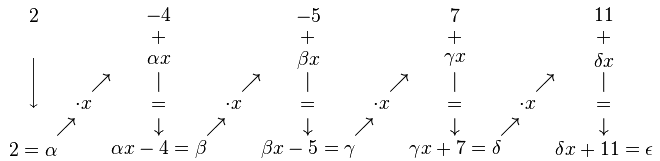
\includegraphics[scale=0.7]{./Images/Hornerschema.png}
			\end{center}
		\end{hint}
\newpage
% !TeX root = ../Main.tex
\section{Folgen}
		\begin{definition}[Konvergenz] \hfill
			\begin{enumerate}
				\item Die Folge $(a_n)_{n \in \mathbb{N}}$ \highlight{konvergiert} gegen $a$ für $n \to \infty$, falls gilt
				$$ \forall \varepsilon > 0 \, \exists n_0 \in \mathbb{N} \, \forall n \geq n_0 \, : \, \abs{a_n - a} < \varepsilon , \qquad a = \lim\limits_{n \to \infty} a_n $$
			\end{enumerate}
		\end{definition}
		\begin{proofhelp} \hfill
			\begin{itemize}
				\item Kein eindeutiger Grenzwert $\Rightarrow$ $(a_n)$ konvergiert nicht.
				\item $(a_n)$ unbeschränkt $\Rightarrow$ $(a_n)$ konvergiert nicht.
			\end{itemize}
		\end{proofhelp}
		\begin{theorem}[Rechenregeln]
			Seien $(a_n)$ und $(b_n)$ konvergente Folgen mit den Grenzwerten $a, b$. Es gilt:
			\begin{enumerate}
				\item $\lim\limits_{n \to \infty} (a_n + b_n) = a + b$
				\item $\lim\limits_{n \to \infty} (a_n - b_n) = a - b$
				\item $\lim\limits_{n \to \infty} (a_n \cdot b_n) = a \cdot b$
				\item Falls zusätzlich $b_n \neq 0 \neq b$, so gilt auch $\lim\limits_{n \to \infty} (a_n / b_n) = a / b$
				\item Falls $ \forall n \, : \, a_n \leq b_n$, so auch $a \leq b$
			\end{enumerate}
		\end{theorem}
	
	\begin{multicols}{2}
		\begin{theorem}[Monotone Konvergenz]
			Sei $(a_n) \subset \mathbb{R}$ nach oben beschränkt und monoton wachsend. Dann ist $(a_n)$ konvergent und $ \lim\limits_{n \to \infty} a_n = \sup\limits_{n \in \mathbb{N}} a_n$
		\end{theorem}
		\begin{proofhelp}[Sandwich-Prinzip]
			Um zu zeigen, dass eine Folge $(a_n)$ konvergiert, finde 2 Folgen $(b_n), (c_n)$ mit identischem Grenzwert $a$, so dass $\forall n \, : \, b_n \leq a_n \leq c_n$ gilt.
		\end{proofhelp}
		\\[1em]
		\begin{definition}[Teilfolge]
			Eine Teilfolge ist eine \highlight{unendliche} Teilmenge einer Folge.
		\end{definition}
		\begin{definition}[Häufungspunkt]
			$a \in \mathbb{R}$ heisst Häufungspunkt, falls die Folge eine gegen $a$ konvergente Teilfolge besitzt.
		\end{definition}
		\begin{theorem}[Bolzano Weierstrass]
			Jede beschränkte Folge besitzt eine konvergente Teilfolge, also auch einen Häufungspunkt. \\[1em]
			Sei $(a_n)$ beschränkt, $a_- = \liminf\limits_{n \to \infty} a_n$, $a_+ = \limsup\limits_{n \to \infty} a_n$. Folgende Aussagen sind äquivalent:
			\begin{enumerate}
				\item $a_n$ konvergiert gegen $a$
				\item Jede Teilfolge von $a_n$ konvergiert gegen $a$
				\item $a_- = a_+$
			\end{enumerate}
		\end{theorem}
		\begin{definition}[Cauchy-Folge]
			$(a_n)$ heisst Cauchy-Folge, falls gilt:
			$$ \forall \varepsilon > 0 \, \exists n_0 \, \forall n,l \geq n_0 \, : \, \abs{a_n - a_l} < \varepsilon $$
		\end{definition}
		\begin{theorem}[Cauchy-Kriterium]
			Für $(a_n)$ sind folgende Aussagen äquivalent:
			\begin{enumerate}
				\item $(a_n)$ ist konvergent.
				\item $(a_n)$ ist Cauchy-Folge.
			\end{enumerate}
		\end{theorem}
		\\[1em]
		\begin{shortcut}
			$$ \lim\limits_{n \to \infty} \sqrt[n]{n} = 1$$
			$$ \lim\limits_{n \to \infty} n^p q^n = 0, \quad n \in \mathbb{N}, q \in (0,1) $$
			$$ \lim\limits_{n \to \infty} \left( 1 + \frac{1}{n} \right)^n = \emath$$
		\end{shortcut}
		\\[1em]
		\begin{definition}[Konvergenz in $\mathbb{R}^2$]
			Eine Folge in $\mathbb{R}^n$ konvergiert, wenn $a_n$ komponentenweise konvergiert.
		\end{definition}
		
	\end{multicols}
\newpage
% !TeX root = ../Main.tex
\section{Reihen} 
	\begin{definition}
		Eine \highlight{Reihe} ist eine Folge der Partialsummen.
	\end{definition}
		\begin{shortcut} \hfill
			\begin{itemize}
				\item Die geometrische Reihe $ \sum\limits_{k = 0}^{\infty} q^k $ konvergiert für $\abs{q} < 1$ gegen $\frac{1}{1-q}$. $ \left( \sum\limits_{k = 0}^{n} q^k \text{ konvergiert für } \abs{q} \neq 1 \text{ gegen } \frac{1-q^{n+1}}{1-q} \right)$
				\item Die harmonische Reihe $ \sum\limits_{k = 0}^{\infty} \frac{1}{k} $ divergiert.
				\item Die alterniernede harmonische Reihe $ \sum\limits_{k = 0}^{\infty} \frac{(-1)^{k + 1}}{k} $ konvergiert gegen $ \log 2$
				\item Die Zeta-Funktion $ \zeta(\alpha) = \sum\limits_{n = 1}^{\infty} \frac{1}{n^\alpha}$ konvergiert für $\alpha > 1$ und divergiert für $\alpha \leq 1$
			\end{itemize}
		\end{shortcut}
	\begin{multicols}{2}
		\begin{theorem}[Nullfolge]
			$$ \lim\limits_{k \to \infty} a_k \neq 0 \quad\Rightarrow\quad \sum\limits_{k = 0}^{\infty} a_k \text{ divergiert.}$$
		\end{theorem}
		\begin{theorem}[Leibnitz-Kriterium]\hfill\\
			Sei $(a_n)$ eine monoton fallend oder wachsende, reelle Nullfolge. Dann konvergiert die altenierende Reihe.
		\end{theorem}
		\begin{theorem}[Cauchy-Kriterium]\hfill\\
			 Die Reihe $\sum\limits_{k = 0}^{\infty} a_k$ ist konvergent, genau dann wann $$\forall \varepsilon > 0 \, \exists n_0 \, : \,  \left\vert \sum\limits_{k = n}^m a_k \right\vert < \varepsilon \quad n,m > n_0 $$
		\end{theorem}
		\begin{theorem}[Majorantenkriterium]\hfill\\
			Seien $\sum\limits_{k = 0}^{\infty} a_k, \sum\limits_{k = 0}^{\infty} b_k$ Reihen, so dass
			\begin{enumerate}
				\item $\exists k_0 \, \forall k \geq k_0 \, : \, \abs{a_k} \leq b_k$
				\item $\sum\limits_{k = 0}^{\infty} b_k$ konvergiert
			\end{enumerate}
			so konvergiert auch $\sum\limits_{k = 0}^{\infty} a_k$\\
			Analog funktioniert das \highlight{Minorantenkriterium} um Divergenz zu zeigen.
		\end{theorem}
		\begin{theorem}[Quotientenkriterium]\hfill\\
			Sei $\forall k \, : \, a_k \neq 0$ 
			\begin{enumerate}
				\item Falls $ \limsup\limits_{k \to \infty} \abs{\frac{a_{k+1}}{a_k}} < 1 $, so ist $\sum\limits_{k = 0}^{\infty} a_k$ konvergent.
				\item Falls $ \liminf\limits_{k \to \infty} \abs{\frac{a_{k+1}}{a_k}} > 1 $, so ist $\sum\limits_{k = 0}^{\infty} a_k$ divergent.
			\end{enumerate}
			Es handelt sich sogar um absolute Konvergenz.
		\end{theorem}
		\begin{theorem}[Wurzelkriterium]\hfill\\
			Sei $(a_k)$ eine Folge in $\mathbb{R}$ oder $\mathbb{C}$
			\begin{enumerate}
				\item Falls $ \limsup\limits_{k \to \infty} \sqrt[k]{\abs{a_k}} < 1 $, so konvergiert $\sum\limits_{k = 0}^{\infty} a_k$.
				\item Falls $ \limsup\limits_{k \to \infty} \sqrt[k]{\abs{a_k}} > 1 $, so divergiert $\sum\limits_{k = 0}^{\infty} a_k$.
			\end{enumerate}
			Es handelt sich sogar um absolute Konvergenz.
		\end{theorem}
		\begin{theorem}[Integral]
			Sei $f:[1,\infty) \to \mathbb{R}^+$ monoton fallend. Dann konvergiert $\sum\limits_{k = 1}^{\infty}f(k)$ genau dann, wenn $\int\limits_{1}^{\infty}f(x) \d x$ existiert. Es gilt:
			$$ 0 \leq \sum\limits_{k = 1}^{\infty}f(k) - \int\limits_{1}^{\infty}f(x) \d x \leq f(1)$$
		\end{theorem}
		\\[1em]
		\begin{theorem}[Konvergenzradius]
			Die Potenzreihe $p(z) = \sum\limits_{k = 0}^{\infty} c_k z^k$ hat den Konvergenzradius $\rho$:
			$$ \rho = \frac{1}{\limsup\limits_{k \to \infty} \sqrt[k]{\abs{c_k}}} $$
			oder einfacher (falls der Grenzwert existiert)
			$$ \rho = \lim\limits_{k \to \infty} \abs{\frac{a_k}{a_{k + 1}}} $$
			D.h. $\abs{z} < \rho \Rightarrow p(z)$ konvergiert.
		\end{theorem}
		\\[1em]
		\begin{definition}[Absolute Konvergenz]\hfill\\
			Die Reihe $\sum\limits_{k = 0}^{\infty} a_k$ konvergiert absolut, falls $\sum\limits_{k = 0}^{\infty} \abs{a_k}$ konvergiert.\\
			Konvergiert eine Folge absolut, so können die Terme in beliebiger Reihenfolge summiert werden.
		\end{definition}
\end{multicols}		
% !TeX root = ../Main.tex
\section{Stetigkeit}
\begin{multicols}{2}
	\begin{definition}[Grenzwert einer Funktion]\hfill\\
		Eine Funktion $f$ hat int $x$ den Grenzwert $a$, falls für \highlight{jede} Folge $(x_n)$ mit $x_n \in \Omega$ und Grenzwert $x$ die Folge $(f(x_n))$ gegen a konvergiert.
	\end{definition}
	\begin{hint}
		Grenzwerte von Funktionen können mit folgenden Tricks evtl. einfacher gezeigt werden, als via $\varepsilon$-$\delta$ Kriterium oder der Definition: 
		\begin{enumerate}
			\item Benutze eine Taylorreihenentwicklung. Für $x \to 0$ können Terme wie $x^5 - x^7 \cdots$ mittles der $\mathcal{O}$-Notation abgeschätzt werden.
			\item Benutze $\lim f(x) = \lim \emath ^{\log f(x)} = \emath ^{\lim \log f(x)}$
			\item Benutze Bernoulli de l'Hôpital falls möglich.
		\end{enumerate}
	\end{hint}
	\\[1em]
	\begin{definition}[Stetigkeit]\hfill\\
		Eine Funktion $f$ ist an der Stelle $x_0$ stetig, falls 
		\begin{enumerate}
			\item $f(x_0)$ definiert ist.				
			\item $\lim\limits_{x \to x_0} f(x)$ existiert.
			\item $\lim\limits_{x \to x_0} f(x) = f(x_0) = f(\lim\limits_{x \to x_0} x)$
		\end{enumerate}
		Sind $f$ und $g$ an $x_0$ stetig, so sind auch $f + g, f \cdot g, f \circ g$ und wenn $g(x_0) \neq 0$ auch $f/g$ an $x_0$ stetig. \\ 
		$f$ ist stetig an $x_0$ falls gilt
		$$ \forall \varepsilon > 0 \, \exists \delta > 0 \, \forall x \, : \, \abs{x - x_0} < \delta \Rightarrow \abs{ f(x)-f(x_0) } < \varepsilon $$
	\end{definition}
		\begin{theorem}[Normale Stetigkeit]\hfill\\
			$f: \Omega \subset \mathbb{R}^d \to \mathbb{R}^n $ ist stetig auf $\Omega$ falls gilt:
			\begin{gather*}
				\forall x_0 \in \Omega \, \forall \varepsilon > 0 \, \exists \delta > 0 \, \forall x \in \Omega\, : \\ 
				\abs{x - x_0} < \delta \Rightarrow \abs{ f(x)-f(x_0) } < \varepsilon
			\end{gather*}
		\end{theorem}
		\begin{theorem}[Gleichmässige Stetigkeit]\hfill\\
			$f: \Omega \subset \mathbb{R}^d \to \mathbb{R}^n $ ist gleichmässig stetig auf $\Omega$ falls gilt:
			\begin{gather*}
				\forall \varepsilon > 0 \, \exists \delta > 0 \, \forall x, x_0 \in \Omega\, : \\ 
				\abs{x - x_0} < \delta \Rightarrow \abs{ f(x)-f(x_0) } < \varepsilon
			\end{gather*}
		\end{theorem}
		\begin{proofhelp}
			Ist f auf einer kompakten Menge $K = \left[ a,b \right]$ stetig, so ist f auf $K$ gleichmässig stetig.
		\end{proofhelp}
		\begin{theorem}[Lipschitz Stetigkeit]\hfill\\
			$f: \Omega \subset \mathbb{R}^d \to \mathbb{R}^n $ ist Lipschitz stetig auf $\Omega$ mit Lipschitzkonstante L falls gilt:
			$$ \exists L \in \mathbb{R}^+ \, \forall x, x_0 \in \Omega \, : \, \norm{ f(x)-f(x_0) } \leq L \norm{x - x_0} $$
		\end{theorem}
		\begin{proofhelp}
			Ist $f$ Lipschitz stetig, so ist $f$ gleichmässig stetig.
		\end{proofhelp}
		\begin{proofhelp}
			$f: \left[ a,b \right] \to \mathbb{R}$ ist stetig $\Rightarrow$ $f(\left[ a,b \right])$ ist beschränkt und nimmt sein Infimum und Supremum an.
		\end{proofhelp}
		\\[1em]
		\begin{theorem}[Zwischenwertsatz]
			\begin{center}
				$a < b, f:\left[ a, b \right] \to \mathbb{R}$ stetig mit $f(a) < f(b)$ $\Rightarrow$ $ \forall y \in \left[ f(a), f(b) \right] \, \exists c \in \left[ a, b \right] \, : f(c) = y$
			\end{center}
		\end{theorem}
		\begin{theorem}
			$f:\left[ a, b \right] \to \mathbb{R}$ stetig und streng monoton $\Rightarrow$ $\Image (f) = [c,d] = [f(a),f(b)]$ oder umgekehrt, $f:[a,b] \to [c,d]$ ist bijektiv und $f^{-1} : [c,d] \to [a,b]$ ist stetig.
		\end{theorem}
		\\[1em]
		\begin{definition}[Punktweise Konvergenz]
			Sei $(f_n)$ eine Folge von Funktionen und sei $f$ eine weitere Funktion. $(f_n)$ \highlight{konvergiert punktweise} gegen $f$ falls:
			$$ \forall x \in \Omega \, : \,  \lim\limits_{n \to \infty} f_n (x) = f(x) $$
		\end{definition}
		\begin{theorem}
			Obige Definition ist äquivalent zu:
			$$ \forall \varepsilon > 0 \, \forall x \in \Omega \, \exists n_0 \in \mathbb{N} \, \forall n \geq n_0 \, : \, \abs{f_n (x) - f(x)} < \varepsilon $$
		\end{theorem}
		\begin{definition}[Gleichmässige Konvergenz]
			Sei $(f_n)$ eine Folge von Funktionen und sei $f$ eine weitere Funktion.$(f_n)$ \highlight{konvergiert gleichmässig} gegen $f$ falls:
			$$ \lim\limits_{k \to \infty} \sup\limits_{x \in \Omega} \abs{f_n(x) - f(x)} = 0$$
		\end{definition}
		\begin{theorem}
			Obige Definition ist äquivalent zu:
			$$ \forall \varepsilon > 0 \, \exists n_0 \in \mathbb{N} \, \forall x \in \Omega \, \forall n \geq n_0 \, : \, \abs{f_n (x) - f(x)} < \varepsilon $$
		\end{theorem}
		\begin{proofhelp}
			Gleichmässige Konvergenz kann gezeigt werden, indem auf kompakten Intervallen für stetige $f_n$ $\sup$ durch $\max$ ersetzt wird. 
			Dann kann das Maximum im Inneren mit der Ableitung gefunden werden und die Randbereiche noch separat untersucht werden.
		\end{proofhelp}
		\begin{theorem}
			Wenn $(f_n) \xrightarrow{glm.} f$ und alle $f_n$ stetig, so ist $f$ auch stetig.
		\end{theorem}
		\begin{corollary}
			Potenzreihen sind stetig im Inneren ihres Konvergenzkreises.
		\end{corollary}
\end{multicols}
% !TeX root = ../Main.tex
\section{Differentialrechung auf $\mathbb{R}$}
	\begin{definition}[Diffenenzierbarkeit] 
		Sei $\Omega \subset \mathbb{R}$ offen, $f: \Omega \to \mathbb{R}, x_0 \in \Omega$
		\begin{enumerate}
			\item f heisst \highlight{differenzierbar} an der Stelle $x_0$ falls 
			$$ \diff{f}{x}(x_0) := f^\prime (x_0) := \lim\limits_{x \to x_0} \frac{f(x)- f(x_0)}{x- x_0}$$ 
			existiert.
			\item $f = (f_1, \dots, f_n): \Omega \to \mathbb{R}^n$ heisst differenzierbar an der Stelle $x_0$ falls jede Komponentenfunktion $f_i$ an $x_0$ differenzierbar ist und $f^\prime(x_0) = (f_1^\prime(x_0), \dots , f_n^\prime(x_0))$
			\item $f$ heisst auf $\Omega$ differenzierbar, falls f an jeder Stelle $x_0 \in \Omega$ differenzierbar ist.
		\end{enumerate}
	\end{definition}
	\begin{proofhelp}
		Differenzierbarkeit $\Rightarrow$ Stetigkeit.
	\end{proofhelp}
	\begin{hint}
		Um Differenzierbarkeit zu zeigen, verwende die Definition und leite \highlight{nicht} einfach ab. \\
		Um stetige Differenzierbarkeit zu zeigen, leite ab und überprüfe auf Stetigkeit.
	\end{hint}
	\\[1em]
	\begin{theorem}[Rechenregeln]
		Sind $f,g: \Omega \to \mathbb{R}$ an der Stelle $x_0 \in \Omega$ differenzierbar, so sind auch $f + g, f \cdot g, f \circ g$ und falls $g(x_0) \neq 0$ auch $f/g$ an $x_0$ stetig.
	\end{theorem}
	\begin{theorem}[Summenregel]
		Seien $f,g: \Omega \to \mathbb{R}$ an $x_0 \in \Omega$ differenzierbar. Es gilt:
		$$ (f + g)^\prime(x_0) = f^\prime(x_0) + g^\prime(x_0) $$
	\end{theorem}
	\begin{theorem}[Produktregel]
		Seien $f,g: \Omega \to \mathbb{R}$ an $x_0 \in \Omega$ differenzierbar. Es gilt:
		$$ (f \cdot g)^\prime(x_0) = f^\prime(x_0) \cdot g(x_0) + f(x_0) \cdot g^\prime(x_0) $$
	\end{theorem}
	\begin{theorem}[Quotientenregel]
		Seien $f,g: \Omega \to \mathbb{R}$ an $x_0 \in \Omega$ differenzierbar und $g(x_0) \neq 0$. Es gilt:
		$$ (f / g)^\prime(x_0) = \frac{f^\prime(x_0) \cdot g(x_0) - f(x_0) \cdot g^\prime(x_0)}{(g(x_0))^2} $$
	\end{theorem}
	\begin{theorem}[Kettenregel]
		Seien $f: \Omega \to \mathbb{R}$ an $x_0 \in \Omega$, $g: \mathbb{R} \to \mathbb{R}$ an $f(x_0)$ differenzierbar. Es gilt:
		$$ (g \circ f)^\prime(x_0) = g^\prime(f(x_0)) \cdot f^\prime(x_0) $$
	\end{theorem}
	\begin{hint}[Ableitung von Potenzfunktionen]
		\hfill\\
		Um $f(x) = g(x)^{h(x)}$ abzuleiten, benütze folgende Umformung:
		$$ f(x) = \exp \left( h(x) \cdot \log (g(x)) \right) \quad\Rightarrow\quad f^\prime(x) =  \left( h^\prime(x) \log (g(x)) + h(x) \frac{g^\prime(x)}{g(x)}\right)g(x)^{h(x)}$$
	\end{hint}
	\\[1em]
		\begin{theorem}[Mittelwertsatz]
			Seien $ -\infty < a < b < \infty, f: [a,b] \to \mathbb{R}$ stetig und in $(a,b)$ differenzierbar. Dann existiert ein $\xi \in (a,b)$ mit
			$$ f^\prime(\xi) = \frac{f(b) - f(a)}{b - a} $$
		\end{theorem}
		\begin{corollary}[Bernoulli de l'Hôpital]
			Seien $f,g: [a,b] \to \mathbb{R}$ stetig und in $(a,b)$ differenzierbar mit $\forall x \in (a,b) \, : \, g^\prime(x) \neq 0$. Sind $f(a) = g(a) = 0$ oder beide Funktionen divergieren bestimmt (gegen $\infty$ oder $-\infty$) und
			$$ \lim\limits_{x \downarrow a} \frac{f^\prime(x)}{g^\prime(x)} $$
			existiert, so gilt
			$$ \lim\limits_{x \downarrow a} \frac{f(x)}{g(x)} = \lim\limits_{x \downarrow a} \frac{f^\prime(x)}{g^\prime(x)} $$
		\end{corollary}
		\begin{theorem}[Umkehrsatz]
			Sei $f: (a,b) \to \mathbb{R}$ differenzierbar mit $f^\prime > 0$ auf $(a,b)$ und seien
			$$ -\infty \leq c = \inf\limits_{a<x<b} f(x) < \sup\limits_{a<x<b} f(x) = d \leq \infty $$
			dann ist f bijektiv und die Umkehrfunktion $f^{-1}: (c,d) \to \mathbb{R}$ ist differenzierbar mit
			$$ \forall x \in (a,b) \, : \, \left(f^{-1}\right)^\prime(f(x)) = \left(f^\prime(x)\right)^{-1} $$
			bzw.
			$$ \forall y \in (c,d) \, : \, \left(f^{-1}\right)^\prime(y) =  \frac{1}{f^\prime(f^{-1}(y))}$$
		\end{theorem}
	\\[1em]
		\begin{definition}[Taylorpolynom]
			Das n-te Taylorpolynom an der Entwicklungsstelle $a$ ist definiert als
			$$ T_n f(x;a) = \sum\limits_{k = 0}^{n} \frac{f^{(k)}(a)}{k!}(x-a)^k = f(a) + \frac{f^\prime(a)}{1!}(x-a) + \frac{f^{\prime\prime}(a)}{2!}(x-a)^2 + \cdots + \frac{f^{(n)}(a)}{n!} (x- a)^n $$
		\end{definition}
		\begin{definition}[Taylor-Formel]
			Sei $f \in C^{m-1}([a,x])$ auf $(a,x)$ m-mal differenzierbar. Dann gibt es $\xi \in (a,x)$ mit
			$$ f(x) = T_{m-1}(x;a) + f^{(m)}(\xi)\frac{(x-a)^m}{m!} $$
			$$ R_n f(x;a) = f^{(n+1)}(\xi)\frac{(x-a)^{n+1}}{(n+1)!} $$
		\end{definition}
		\begin{proofhelp}[Restterm]
			Für den Restterm gilt:
			$$ \lim\limits_{x \to a} \frac{R_n f(x;a)}{(x-a)^n} = 0 $$
		\end{proofhelp}
		\begin{proofhelp}[Restterm nach Integralrechnung]
			$$R_n f(x;a) = \frac{1}{n!}\int\limits_{a}^{x}(x-t)^n f^{(n+1)}(t) \d t$$
		\end{proofhelp}
	\\[1em]
		\begin{theorem}[Extremalstellen]
			\hfill\\
			Sei $\Omega \subset \mathbb{R}, f: \Omega \to \mathbb{R}, f \in C^{\infty}(\Omega), x_0 \in \Omega$. Einer der folgenden Fälle tritt ein:
			\begin{enumerate}
				\item $\forall j \geq 1 \, : \, f^{(j)}(x_0) = 0$
				\item $m := 1 + \max \{ j : f^{(i)}(x_0) = 0, 1 \leq i \leq j \}$ d.h $f^{(m)}(x_0) \neq 0$ und $f^{(1)}(x_0) = \dots = f^{(m - 1)}(x_0) = 0$
				\begin{enumerate}
					\item m ist ungerade, dann ist $x_0$ keine Extremalstelle.
					\item m ist gerade und $f^{(m)}(x_0) > 0$, dann ist $x_0$ eine strikte lokale Minimalstelle.
					\item m ist gerade und $f^{(m)}(x_0) < 0$, dann ist $x_0$ eine strikte lokale Maximalstelle.
				\end{enumerate}
			\end{enumerate}
		\end{theorem}
% !TeX root = ../Main.tex
\section{Integralrechung auf $\mathbb{R}$}
	\subsection{Riemannintegral}
		\begin{definition}[Partition]
			\hfill
			\begin{enumerate}
				\item Eine \highlight{Partition} eines Intervalles $[a,b]$ ist eine endliche Menge von Punkten
				$$ P = \{ a = x_0, x_1, x_2, \dots, x_n = b \}, \quad x_0 < x_1 < x_2 < \dots < x_n$$
				\item $\mathscr{P}(I)$ bezeichnet die Menge aller Partitionen eines Intervalls $I$. 
				\item Die Feinheit ist definiert als $\delta(P) := \max\limits_{1\leq i \leq n} (x_i - x_{i - 1}) = $ Länge des grösste Teilintervalls $I_i:= [x_{i-1}, x_i]$.
			\end{enumerate}
		\end{definition}
		\begin{definition}[Riemannsumme]
			\hfill\\
			$\xi$ ist eine Wahl von Zwischenpunkten einer Partition, $x_{i-1} \leq \xi_i \leq x_i, 1 \leq i \leq n$ \\
			Sei $f:[a,b] \to \mathbb{R}$ eine beschränkte Funktion \\
			Jede Summe der Form $S(f,P,\xi) := \sum\limits_{i = 1}^{n} f(\xi_i)(x_{i}-x_{i-1})$ nennt man \highlight{Riemansumme}. \\
			Die Summe $U(f,P) := \sum\limits_{i = 1}^{n} (\inf\limits_{I_i}f)(x_{i}-x_{i-1})$ heisst Untersumme. \\
			Die Summe $O(f,P) := \sum\limits_{i = 1}^{n} (\sup\limits_{I_i}f)(x_{i}-x_{i-1})$ heisst Obersumme. \\
		\end{definition}
		\begin{proofhelp}
			$P,Q \in \mathscr{P}(I), P \subset Q \quad\Rightarrow\quad U(f,P) \leq U(f,Q) \leq O(f,Q) \leq O(f,P)$
		\end{proofhelp}
		\begin{definition}[Riemann-integrierbar]
			Für eine beschränkte Funktion $f:I \to \mathbb{R}$ bezeichnen:
			$$\underline{\int\limits_{a}^{b}}f(x)\d x := \sup\limits_{P \in \mathscr{P}(I)} U(f,P) \qquad \overline{\int\limits_{a}^{b}}f(x)\d x := \inf\limits_{P \in \mathscr{P}(I)} O(f,P)$$
			$f$ heisst \highlight{Riemann-integrierbar}, falls 
			$$ \underline{\int\limits_{a}^{b}}f(x)\d x = \overline{\int\limits_{a}^{b}}f(x)\d x$$ 
		\end{definition}
		\begin{theorem}
			Sei $f:I \to \mathbb{R}$ beschränkt. Folgende Aussagen sind äquivalent:
			\begin{enumerate}
				\item $f(x)$ ist integrierbar über $I$
				\item $\forall \varepsilon > 0 \, \exists P \in \mathscr{P}(I) \, : \, O(f,P) - U(f,P) < \varepsilon$
			\end{enumerate}
		\end{theorem}
		\begin{theorem}
			\hfill
			\begin{enumerate}
				\item Jede stetige Funktion ist Riemann-integrierbar
				\item Jede monotone Funktion ist Riemann-integerierbar
			\end{enumerate}
		\end{theorem}
		\\[1em]
		\begin{theorem}[Mittelwertsatz der Integralrechnung]\hfill\\
			Sei $f:[a,b] \to \mathbb{R}$ eine stetige Funktion. Dann existiert ein $\xi \in [a,b]$ mit 
			$$ \int\limits_{a,b} f(x) \d x = (b-a) f(\xi)$$
		\end{theorem}
	\subsection{Hauptsatz der Infinitesimalrechnung}
		\begin{theorem}[Hauptsatz A]
			Sei $f:[a,b] \to \mathbb{R}$ stetig. \\
			Wir definieren: $\forall x \in [a,b] \, : \, F(x) := \int\limits_{a}^x f(t) \d t$ \\
			Dann ist $F(x): I \to \mathbb{R}$ differenzierbar mit $\forall x \in [a,b] \, : \, F^\prime(x) = f(x)$
		\end{theorem}
		\begin{theorem}[Hauptsatz der Differential- und Integralrechnung]
			Sei $f: I \to \mathbb{R}$ stetig und $F$ eine beliebige Stammfunktion von $f$. Dann gilt:
			$$ \int\limits_{a}^b f(x) \d x = F(b) - F(a) =: F(x)\range{a}{b}$$
		\end{theorem}
	\subsection{Integrationsmethoden}
		\begin{proofhelp}[Generelle Regeln]
			%\hfill
			\begin{align*}
				\int f(a + x) \d x &= F(a+x) + c \\
				\int g^\prime(x)g(x) \d x &= \frac{1}{2}g(x)^2 + c \\
				\int \frac{g^\prime(x)}{g(x)} \d x &= \log \abs{g(x)} + c
			\end{align*}
		\end{proofhelp}
		\begin{proofhelp}[Partielle Integration]
			Seien $f,g:[a,b] \to \mathbb{R}$ stetig. Es gilt:
			$$ \int\limits_{a}^{b} f(x)g^\prime(x) \d x = f(x)g(x) \range{a}{b} - \int\limits_a^b f^\prime(x)g(x) \d x $$
		\end{proofhelp}
		\begin{proofhelp}[Substitution]
			Sei $f:[a,b] \to \mathbb{R}$ stetig, $g[c,d] \to [a,b] \in C^1$ Dann gilt:
			$$ \int\limits_{a}^{b} f(g(t)) \cdot g^\prime(t) \d t = \int\limits_{g(a)}^{g(b)}f(x) \d x $$
		\end{proofhelp}
		%\begin{proofhelp}[Partialbruchzerlegung]
		%	Mache mit gebrochenrationaler Funktion ein PBZ und integriere die Summen einzeln. Es gilt dabei:
		%	\begin{align*}
		%		\int \frac{\d x}{(x- x_0)^n} &= \begin{cases} \log\abs{x-x_0} + c & n = 1 \\ \frac{1}{1 - n} \cdot \frac{1}{(x- x_0)^{n - 1}} & n \geq 2 \end{cases} \\
		%		\int \frac{bx + d}{((x-a)^2+b^2)^m} \d x
		%	\end{align*}
		%\end{proofhelp}
	\subsection{Uneigentliches Integral}
		\begin{definition}
			Sei $f$ eine Funktion auf einem Intervall $(a,b)$, deren Einschränkung auf jedes kompakte Teilintervall $[a',b']$ integrierbar ist. Dann ist das uneigentliche Integral von f von a bis b definiert als:
			$$\int\limits_{a}^{b} f(x) \d x := \lim\limits_{a' \downarrow a} \lim\limits_{b' \uparrow b} \int\limits_{a'}^{b'}f(x) \d x$$
			falls diese Grenzwerte existieren.
		\end{definition}
		\begin{proofhelp}
			\highlight{Achtung}, die beiden Grenzen müssen, getrennt untersucht werden!! $\int\limits_{-\infty}^{\infty} x \d x$ existiert nicht.
		\end{proofhelp}
		\begin{hint}
			Hier können Majorantenkriterium und Minorantenkriterium helfen zu entscheiden, ob das Integral existiert.
		\end{hint}
% !TeX root = ../Main.tex
\section{Differentialgleichungen}
	\begin{definition}
		Eine \highlight{Differentialgleichung} ist eine Gleichung für eine Funktion von einer oder mehreren Variablen, in der auch Ableitungen dieser Funktion vorkommen.
	\end{definition}
		\begin{definition}[Lineare Differentialgleichung]
			Eine lineare DGL n-ter Ordnung hat die Gestalt $y^{(n)}(x) + a_{n-1}(x)y^{(n-1)}(x) + \dots + a_0(x) y(x) = b(x)$, mit $a_i(x), b(x)$ Funktionen. 
		\end{definition}
		\subsection{Homogene lineare DGL mit konstanten Koeffizienten}
			\begin{definition}[Charakteristisches Polynom]
				Das charakteristische Polynom der Gleichung $y^{(n)}(x) + a_{n-1}y^{(n-1)}(x) + \dots + a_0y(x) = 0$ (homogene lineare DGL) ist gegeben durch
				$$ p(t) = t^n + a_{n-1} t^{n-1} + \dots + a_0 $$
			\end{definition}
			\begin{proofhelp}
				Um homogene lineare DGL mit konstanten Koeffizienten zu lösen, suche die Nullstellen des charakteristischen Polynoms und schaue unten welche Nullstellen zu welchen Lösungen führen. 
				Die allgemeine Lösung ist die Linearkombination all dieser Lösungen. ($y_{allg}(x) = c_1 \cdot \emath^{\lambda_1 x} \cdots $)
				\begin{enumerate}
					\item Ist $\lambda \in \mathbb{R}$ eine k-fache Nullstelle, so sind $\emath^{\lambda x}, x^1 \cdot \emath^{\lambda x}, \dots, x^{k-1}\emath^{\lambda x}$ Lösungen der DGL.
					\item Sind $\lambda = \alpha + \imath \beta$ und $\overline{\lambda} = \alpha - \imath \beta $ mit $\beta \neq 0$ ein Paar konjugiert komplexer Nullstellen mit Vielfachheit k, so sind 
					$$ \emath^{\alpha x} \sin (\beta x), \quad \emath^{\alpha x} \cos (\beta x), $$
					$$ x^1 \cdot \emath^{\alpha x} \sin (\beta x), \quad x^1 \cdot \emath^{\alpha x} \cos (\beta x), $$
					$$ \vdots $$
					$$ x^{k-1} \cdot \emath^{\alpha x} \sin (\beta x), \quad x^{k-1} \cdot \emath^{\alpha x} \cos (\beta x) $$
					Lösungen der DGL. Beachte, dass die Koeffizienten von $x^{i} \cdot \emath^{\alpha x} \sin (\beta x)$ und $x^{i} \cdot \emath^{\alpha x} \cos (\beta x)$ verschieden sein dürfen.
				\end{enumerate}
			\end{proofhelp}
		\subsection{Inhomogene lineare DGL mit konstanten Koeffizienten}
			\begin{proofhelp}
				Um inhomogene lineare DGL mit konstanten Koeffizienten zu lösen, gehe so vor:
				\begin{enumerate}
					\item Löse die zugehörige homogene DGL und erhalte $y_{h}$.
					\item Mache einen Ansatz vom Typ der rechten Seite und erhalte $y_{s}$.
					\item Kombiniere die Lösung $y_{allg} = y_{h} + y_{s}$.
				\end{enumerate}
			\end{proofhelp}
			\begin{hint}[Ansatz der rechten Seite]
				Finde in der Tabelle den Ansatz. Dieser wird nun in die DGL eingesetzt und so die noch unbekannten Koeffizienten bestimmt.			
			\end{hint}
			\begin{center}
				\begin{tabular}{|C{5cm}|C{8cm}|}
					\hline
					\rowcolor[gray]{0.9}
					\text{Störfunktion}																												&	\text{Ansatz für }y_p														\tabularnewline\hline
					a \cdot \emath^{\mu x}																											&	b \cdot \emath^{\mu x}														\tabularnewline\hline
					a \cdot \sin	 (\nu x)		\linebreak		\fracsize b \cdot \cos ( \nu x)															&	c \cdot \sin (\nu x) + d \cdot \cos (\nu x)									\tabularnewline\hline
					a \cdot \emath^{\mu x} \cdot \sin	 (\nu x)		\linebreak		\fracsize b \cdot \emath^{\mu x} \cdot \cos ( \nu x)				&	\emath^{\mu x} \cdot (c \cdot \sin (\nu x) + d \cdot \cos (\nu x))			\tabularnewline\hline
					P_n(x)																															&	R_n(x)																		\tabularnewline\hline
					P_n(x) \emath^{\mu x} 																											&	R_n(x) \emath^{\mu x}														\tabularnewline\hline
					P_n(x) \cdot \emath^{\mu x} \cdot \sin	 (\nu x)		\linebreak		\fracsize Q_n(x) \cdot \emath^{\mu x} \cdot \cos ( \nu x)		&	\emath^{\mu x} \cdot (R_n(x) \cdot \sin (\nu x) + S_n(x) \cdot \cos (\nu x))	\tabularnewline\hline
				\end{tabular}
			\end{center}
			wobei $P_n(x), R_n(x), Q_n(x)$ und $S_n(x)$ Polynome von Grad $n$ sind.\\[1em]
			\begin{hint}
				Liegt eine Linearkombination der Störfaktoren vor, so hat man auch als Ansatz eine entsprechende Linearkombination zu wählen.
			\end{hint}
			\begin{hint}
				Falls $\lambda = \mu + \imath \nu$ eine m-fache Nullstelle des charakteristischen Polynomes ist, so muss man den Ansatz mit $x^m$ multiplizieren.
			\end{hint}
		\subsection{Lineare DGL erster Ordnung mit allgemeinen Koeffizienten}
			Die lineare DGL hat die allgemeine Form
			$$ y^\prime(x) = a(x)\cdot y + b(x) $$
			\begin{proofhelp}[Homogener Fall]
				Falls $y(x) \neq 0$ gilt $y(x) = \emath^{A(x)}\cdot K, \quad K \in \mathbb{R} - \{0\}$.\\ $A(x)$ ist eine Stammfunktion von $a(x)$.
			\end{proofhelp}
			\begin{proofhelp}[Allgemeiner Fall]
				Die allgemeine Lösung der DGL $ y^\prime(x) = a(x)\cdot y + b(x) $ lautet:
				$$ y_{all}(x) = \emath^{A(x)}\cdot \int \left( b(x) \emath^{-A(x)} \right) \d x + K \cdot \emath^{A(x)} $$
				wobei $K \in \mathbb{R}$ und $A(x)$ eine Stammfunktion von $a(x)$ ist.
			\end{proofhelp}
			\begin{hint}[Variation der Konstanten]
				Dies ist eine Alternative zum Lösungsschema im allgemeinen Fall. \\
				\begin{enumerate}
					\item Ignoriere $b(x)$ und löse den homogenen Fall. Erhalte $y_h(x)$
					\item Bestimme $y_p(x)$ so: $y_p(x) = y_h(x) \cdot \int \frac{b(x)}{y_h(x)} \d x \quad$ (setze $y_h$ mit $K = C(t)$ in die DGL ein).
					\item $y_{allg}(x) = y_h(x) + y_p(x)$
				\end{enumerate}
			\end{hint}
		\subsection{Separierbare DGL}
			\begin{hint}[Sparation der Variablen]
				Eine DGL der Form $y^\prime(x) = f(x)g(y)$ löst man durch Separation der Variablen, d.h. ersetze $y^\prime(x)$ durch $\diff{y}{x}$, integriere beide Seiten und löse nach $y$ auf. Möglicherweise ist hier auch eine Substitution sehr hilfreich.
			\end{hint}
		\subsection{Bernoulli DGL}
			\begin{proofhelp}[Sparation der Variablen]
				Eine DGL der Form $y^\prime(x) = f(x)y + g(x)y^{\alpha}$ löst man durch Substitution. Wähle 
				$$u = y^{1 - \alpha} \Leftrightarrow y = u^{\frac{1}{1-\alpha}}$$
				so erhält man
				$$ u^\prime = \underbrace{(1 - \alpha)f(x)}_{f^*(x)}u + \underbrace{(1 - \alpha) g(x)}_{g^*(x)} $$
				Dies löst man mit dem Ansatz für lineare DGL erster Ordnung mit allgemeinen Koeffizienten.
			\end{proofhelp}
% !TeX root = ../Main.tex
\section{Differentialrechnung in $\mathbb{R}^n$}
	\subsection{Stetigkeit}
		\begin{definition}
			Sei $\Omega \subset \mathbb{R}^n, f: \Omega \to \mathbb{R}, a \in \Omega$
			\begin{enumerate}
				\item $f$ hat den Grenzwert $c \in \mathbb{R}$, falls:
				$$ \forall \varepsilon > 0 \, \exists \delta > 0 \, : \, \abs{x-a} < \delta \Rightarrow \abs{f(x) - c} < \varepsilon$$
				\item $f$ heisst in $a$ stetig, wenn $\lim\limits_{x \to a} f(x) = f(a)$
				\item $f$ heisst in $\Omega$ stetig, wenn $f$ in allen $a \in \Omega$ stetig ist.
			\end{enumerate}
		\end{definition}
		\begin{proofhelp}
			$f$ besitzt keinen Grenzwert in $a$, wenn sich bei Annäherungen an $a$ auf verschiedenen Kurven verschiedene Grenzwerte oder keine Grenzwerte ergeben.
		\end{proofhelp}
		\begin{proofhelp}
			Die Summe, das Produkt und der Quotient (Nenner $\neq 0$) stetiger Funktionen sind stetig.
		\end{proofhelp}
		\begin{proofhelp}[Sandwich-Satz]
			Seien $f,g,h$ Funktionen mit $\forall x \in B_r(a) \, : \, g(x) \leq f(x) \leq h(x)$. Wenn $\lim\limits_{x \to a} g(x) = L =\lim\limits_{x \to a} h(x)$, dann gilt $\lim\limits_{x \to a} f(x) = L$
		\end{proofhelp}
		\begin{hint}[Polarkoordinaten]
			Für Grenzwertbestimmungen ist es oft nützlich, die Funktionen in Polarkoordinaten umzuschreiben. \\
			Für 2-Dimensionale Funktionen gilt $x = r \cos \vartheta , y = r \sin \vartheta$ \\
			Für 3-Dimensionale Funktionen gilt $x = r \sin \vartheta \cos \varphi , y = r \sin \vartheta \sin \varphi , z = r \cos \vartheta $
		\end{hint}
		\begin{hint}[Substitution]
			Man berechnet den Grenzwert $\lim\limits_{(x,y) \to (a,b)} f(g(x,y))$ indem man zunächst den Grenzwert $t_0 = \lim\limits_{(x,y) \to (a,b)} g(x,y)$ bestimmt. Dann bestimmt man $\lim\limits_{t \to t_0} f(t)$.
		\end{hint}
	\subsection{Partielle Differnzierbarkeit}
		\begin{definition}
			$f$ heisst an der Stelle $x_0$ in Richtung $e_i$ (Einheitsvektor) partiell differenzierbar, falls der Limes
			$$ \lim\limits_{h \to 0} \frac{f(x_0 + he_i) - f(x_0)}{h} $$
			existiert. \\
			Achtung: partielle Differenzierbarkeit $\not\Rightarrow$ Stetigkeit.
		\end{definition}
	\subsection{Differenzierbarkeit}
		\begin{definition}
			$f$ heisst an der Stelle $x_0$ differenziebar, falls es eine Abbildung $A: \mathbb{R}^n \to \mathbb{R}$ gibt, so dass
			$$ f(x) = f(x_0) + A \cdot (x - x_0) + R(x_0,x), \qquad \text{wobei } \lim\limits_{x \to x_0} \frac{R(x_0,x)}{\abs{x - x_0}} = 0$$
			In diesem Fall heisst $A$ Differential und wird mit $\d _{x_0}f$ bezeichnet.
		\end{definition}
		\begin{theorem}
			Sei $f: \Omega \to \mathbb{R}$ differenzierbar an $x_0 \in \Omega$ Dann existieren die partiellen Ableitungen und das Differential kann als 
			$$ \d _{x_0} f = \left( \pdiff{f}{x^1}(x_0), \pdiff{f}{x^2}(x_0), \dots ,\pdiff{f}{x^n}(x_0) \right)$$
			dargestellt werden.
		\end{theorem}
		\begin{proofhelp}
			$f$ ist differenzierbar $\Rightarrow$ $f$ ist stetig.
		\end{proofhelp}
		\begin{theorem}
			Existieren die partiellen Ableitungen und sind stetig $\Rightarrow$ f ist differenzierbar.
		\end{theorem}
		\begin{proofhelp}[Untersuchen der Differenzierbarkeit]
			\hfill
			\begin{enumerate}
				\item Ist $f$ in $x_0$ stetig? Wenn nein breche ab.
				\item Ist $f$ in $x_0$ partiell differenzierbar? Wenn nein breche ab.
				\item Sind die partiellen Ableitungen stetig? Wenn ja ist $f \in C^1$, wenn nein fahre fort.
				\item Ist
				$$ \lim\limits_{x \to x_0} \frac{f(x) - f(x_0) - \sum\limits_{i} \pdiff{f}{x^i}(x_0) \left( x^i - x_0^i \right)}{\abs{x - x_0}} = 0 $$
				Wenn ja ist $f$ differenzierbar, wenn nein nicht.
			\end{enumerate}
		\end{proofhelp}
	\subsection{Differentiationsregeln}
		\begin{proofhelp}
			Die Summenregel, Produktregel und Quotientenregel gelten genau wie in $\mathbb{R}$
		\end{proofhelp}
		\begin{theorem}[Kettenregel 1]
			\hfill \\
			Sei $g:\Omega\to\mathbb{R}$ in $x_0 \in\Omega$ differenzierbar. Sei $f:\mathbb{R}\to\mathbb{R}$ an $g(x_0)$ differenzierbar. Es gilt:
			$$ \d (f \circ g)(x_0) = f^\prime(g(x_0)) \cdot \d g(x_0)$$
		\end{theorem}
		\begin{theorem}[Kettenregel 2]
			\hfill \\
			Seien $\Omega \subset \mathbb{R}^n, I \subset \mathbb{R}, g: I \to \Omega, t \mapsto (g_1(t), \dots , g_n(t)), f: \Omega \to \mathbb{R}$, sowie $g$ an $t_0$ und $f$ an $g(t_0)$ differenzierbar. Es gilt:
			$$ \diff{}{t}(f \circ g)(t_0) = \d f(g(t_0)) \cdot g^\prime(t_0)$$
		\end{theorem}
	\subsection{Anwendungen}
		\begin{theorem}[Richtungsableitung]
			Die Ableitung von $f$ an $x_0$ in die Richtung des \highlight{normierten} Richtungsvektors $v$ ist:
			$$ \dotp{\nabla f(x_0)}{v} $$
		\end{theorem}
		\begin{theorem}[Leibnitzregel für Parameterintegrale]
			Für stetig differenzierbare Funktionen $\chi, \varphi, f$ gilt:
			$$ \diff{}{\omega}\int\limits_{\chi(\omega)}^{\varphi(\omega)}f(x, \omega) \d x = \int\limits_{\chi(\omega)}^{\varphi(\omega)} \pdiff{f}{\omega}(x,\omega) \d x + f(\varphi(\omega),\omega)\cdot\varphi^\prime(\omega) - f(\chi(\omega),\omega)\cdot\chi^\prime(\omega)$$
			Dies ist auch für konstante Grenzen anwendbar, dabei fallen die letzten beiden Terme der rechten Seite logischerweise weg.
		\end{theorem}
	\subsection{Gradient}
		\begin{proofhelp}
			Sei $f \in C^1(\Omega), x_0 \in \Omega$. Dann ist $\nabla f(x_0)$ die Richtung und $\abs{\nabla f(x_0)}$ der Betrag des steilsten Anstieges von $f$ an der Stelle $x_0$ \\
			$\nabla f(x_0)$ steht senkrecht zur Niveaufläche von $f$ durch $x_0$
		\end{proofhelp}
	\subsection{Konservative Vektorfelder}
	 	\begin{definition}
		 	Ein Vektorfeld $v$ heisst konservativ, falls alle Wegintegrale entlang geschlossener Wege den Wert 0 haben.
		 \end{definition}
		 \begin{theorem}
		 	Für stetige Vektorfelder gilt:
		 	$$ V \text{ ist konservativ } \Leftrightarrow \exists f \in C^1 \, : \, V = \nabla f$$
		 	In diesem Fall heisst $V$ Potentialfeld und $f$ ist das Potential von $V$.
		 \end{theorem}
		 \begin{proofhelp}
		 	So findet man heraus, ob ein Vektorfeld ein Potential besitzt: 
		 	\begin{enumerate}
		 		\item Nimm die x-Komponente und integriere nach $\d x$. Finde eine Funktion $f$, die noch von einer Konstanten in Abhängigkeit von $y,z$ (falls 3D) abhängt.
		 		\item Nimm die eintstandene Funktion inklusive Konstante und leite nach $y$ ab.
		 		\item Setze nun die Ableitung mit der y-Komponente des Vektorfeldes gleich und bestimme so die Ableitung der Konstante aus Schritt 1 genauer.
		 		\begin{enumerate}
		 			\item Falls die Ableitung der Konstante von x abhängen sollte, brich ab. Das Vektorfeld hat kein Potential.
		 		\end{enumerate}
		 		\item Integriere die Ableitung der Konstanten nach y und bestimme so $f$ genauer (nun bis auf eine Konstante in Abhängigeit von $z$)
		 		\item Leite wieder ab. Bestimme die Ableitung der fehlende Konstante wieder genauer. Falls die Ableitung der Konstanten 0 ist, so melde Erfolg, sonst Misserfolg.
		 	\end{enumerate}
		 \end{proofhelp}
	\subsection{Wegintegrale}
		\begin{definition}
			Das Wegintegral vom Vektorfeld $v$ längs einer Kurve in Parameterdarstellung $\gamma$, so ist das Wegintegral
			$$ \int\limits_{\gamma} \vec{v} \cdot \d \vec{s} = \int\limits_{\gamma} v(\gamma) \d \gamma := \int\limits_{a}^{b} \dotp{v(\gamma(t))}{\gamma^\prime(t)} \d t$$
		\end{definition}
		\begin{proofhelp}[Eigenschaften des Wegintegrales]
			\hfill
			\begin{enumerate}
				\item Ist $\gamma$ nur stückweise $C^1$ und sind es nur endlich viele Teilstücke, so summieren wir einfach über die Teilstücke um das Wegintegral zu erhalten.
				\item Das Wegintegral hängt nicht von der parametrisierung des Weges ab.
				\item Für den selben Weg rückwärts ändert sich nur das Vorzeichen des Integerals.
				\item Ist $V$ ein Vektorfeld mit Potential $f: \Omega \to \mathbb{R}$ und $\gamma: [a,b] \to \Omega$ der Weg, so gilt:
				$$ \int\limits_{\gamma} V \d s = \int\limits_{\gamma} \d f = f(\gamma(b)) - f(\gamma(a)) $$
			\end{enumerate}
		\end{proofhelp}
	\subsection{Höhere Ableitungen}
		\begin{theorem}[Satz von Schwarz]
			Ist $f \in C^k(\Omega)$ so sind alle partiellen Ableitungen vom Grad $\leq$ k von der Reihenfolge der Ableitungen unabhängig.
		\end{theorem}
	\subsection{Rotation}
		\begin{definition}
			Sei $V : \Omega \to \mathbb{R}^2$ ein Vektorfeld. Die skalare Rotation ist 
			$$ \Rot(V) := \pdiff{v^2}{x} - \pdiff{v^1}{y} $$ 
		\end{definition}			
		\begin{proofhelp}
			$\Rot(V) = 0$ ist notwendige Bedingung, damit ein Potential existieren kann.
			$\Rot(V) = 0$ ist hinreichend, falls das Gebiet einfachzusammenhängend ist, d.h. keine Löcher enthält. Zudem muss $V$ stetig sein. Exaktere Definition von einfachzusammenhängend: Wegzusammenhängend und jeder geschlossene Weg lässt sich auf einen Punkt zusammenziehen.
		\end{proofhelp}
		\begin{definition}
			Sei $V : \mathbb{R}^3 \to \mathbb{R}^3$ ein Vektorfeld. Es gilt
			$$ \Rot(V) := \nabla \times V = 
			\begin{pmatrix}
				\pdiff{V_3}{y}-\pdiff{V_2}{z} \\[1ex]
				\pdiff{V_1}{z}-\pdiff{V_3}{x} \\[1ex]
				\pdiff{V_2}{x}-\pdiff{V_1}{y} 
			\end{pmatrix}			 $$ 
		\end{definition}	
	\subsection{Divergenz}
		\begin{definition}
			Sei $V : \mathbb{R}^3 \to \mathbb{R}^3$ ein Vektorfeld. Es gilt
			$$ \div(V) := \nabla \cdot V = \pdiff{V_1}{x} + \pdiff{V_2}{y} + \pdiff{V_3}{z} $$ 
		\end{definition}	
	\subsection{Quadratische Näherung in $\mathbb{R}^n$}
		\begin{proofhelp}
			Sei $f: \mathbb{R}^n \to \mathbb{R}$ eine $C^2$-Funktion, sowie $x_0,x_1 \in \mathbb{R}^n$
			Die quadratische Näherung von $f$ lautet:
			$$
				f(x_1) = f(x_0) + \nabla f(x_0) (x_1 - x_0) + \frac{1}{2}(x_1 - x_0)(\nabla^2f(x_0))(x_1 -x_0)^T + r
			$$
		\end{proofhelp}
		\begin{proofhelp}[Hessematrix]
			Die Hessemathrix von f $\nabla^2f$ lautet:
			$$ 
			\nabla^2f = 
			\begin{pmatrix}
			\pdiff{f^2}{x^1\partial x^1} 	& \cdots & \pdiff{f^2}{x^1\partial x^n} \\
			\vdots							& \ddots & \vdots						\\
			\pdiff{f^2}{x^n\partial x^1} 	& \cdots & \pdiff{f^2}{x^n\partial x^n} \\
			\end{pmatrix}
			$$
		\end{proofhelp}
	\subsection{Extema}
		\begin{definition}
			Ein Punkt $x_0 \in \mathbb{R}^n$ mit $ \d f(x_0) = 0$ heisst kritischer Punkt von f.
		\end{definition}
		\begin{proofhelp}
			Sei $x_0$ ein kritischer Punkt.
			\begin{enumerate}
				\item Falls $\nabla^2f(x_0)$ positiv definit ist, so ist $x_0$ ein lokales Minimum. (Alle Eigenwerte > 0)
				\item Falls $\nabla^2f(x_0)$ negativ definit ist, so ist $x_0$ ein lokales Maximum. (Alle Eigenwerte < 0)
				\item Falls $\nabla^2f(x_0)$ indefinit, so ist $x_0$ ein Sattelpunkt.	(Eigenwerte > 0 und < 0)
				\item Falls $\nabla^2f(x_0)$ singulär, ist der kritische Punkt entartet.
			\end{enumerate}
		\end{proofhelp}		
	\subsection{Vektorwertige Funktionen}
		Sei $\Omega \subset \mathbb{R}^n, f = (f^i) : \mathbb{R}^n \to \mathbb{R}^l, f^i : \Omega \to \mathbb{R}$ \\
		\begin{definition}
			$f$ heisst differenzierbar, wenn jede Komponente differenzierbar ist.
		\end{definition}
		\begin{proofhelp}[Jacobi-Matrix]
			Die Jacobi-Matrix ist eine Darstellung des Differentials von f:
			$$
			\d f(x_0) = 
				\begin{pmatrix}
					\pdiff{f^1}{x^1}(x_0) 	& \cdots & \pdiff{f^1}{x^n}(x_0) \\
					\vdots					& \ddots & \vdots				\\
					\pdiff{f^l}{x^1}(x_0)	& \cdots & \pdiff{f^l}{x^n}(x_0) \\
				\end{pmatrix}
			$$
		\end{proofhelp}
		\begin{proofhelp}[Regeln]
			\hfill
			\begin{enumerate}
				\item Für Multiplikation mit Skalar und Addition zweier Funktionen verhält sich dieses Differential identisch wie das in einer Dimension.
				\item Für das Skalarprodukt gilt:
				$$ 
					\d (\dotp{f}{g})(x_0) = \dotp{f(x_0)}{(\d g)(x_0)} + \dotp{(\d f)(x_0)}{g(x_0)}, \quad\text{ wobei } \dotp{f(x_0)}{(\d g)(x_0)} = \sum\limits_{i=1}^{l}(f^i(x_0)\cdot (\d g^i)(x_0))
				$$
			\end{enumerate}
		\end{proofhelp}
		\begin{proofhelp}[Kettenregel]
			Die Kettenregel gilt wie im 1D Fall, nur dass hier Matrixmultiplikationen durchgeführt werden müssen.
		\end{proofhelp}
% !TeX root = ../Main.tex
\section{Integralrechnung in $\mathbb{R}^n$}
	\subsection{$\mathbb{R}^2$}
		In $\mathbb{R}^2$ leiten wir das Integral über einem Rechteck analog zum Fall in $\mathbb{R}$ her. Wir zerlegen das Rechteck in Teilrechtecke, wählen in den Teilrechtecken je einen Zwischenpunkt und summieren auf. \\
		\begin{theorem}[Fubini]
			Sei $Q = [a,b]\times[c,d] \subset \mathbb{R}^2$ und $f \in C^0(Q)$ Dann gilt:
			$$ \iint\limits_{Q} f \d \mu = \int\limits_a^b\left(\int\limits_c^d f(x,y)\cdot \d y \right) \d x = \int\limits_c^d\left(\int\limits_a^b f(x,y)\cdot \d x \right) \d y
			$$
		\end{theorem}
		\\[1em]
		\begin{definition}[Normbereich]
			$D \subset \mathbb{R}^2$ heisst Normbereich bezgl. der x-Achse bzw. y-Achse falls es stetige Funktionen $f,g$ bzw. $\overline{f}, \overline{g}$ gibt mit
			$$ D = \{(x,y) \vert a \leq x \leq b \wedge g(x) \leq y \leq h(x)\} \quad\text{bzw.}\quad D = \{(x,y) \vert \overline{a} \leq y \leq \overline{b} \wedge \overline{g}(y) \leq x \leq \overline{h}(y)\} $$
		\end{definition}
		\begin{theorem}[Integration über Normbereich]
			Sei $f$ stetig auf einem Normalbereich
			\begin{enumerate}
				\item $D = \{(x,y) \vert a \leq x \leq b \wedge g(x) \leq y \leq h(x)\}$, so gilt:
				$$ \iint\limits_{D} f \d \mu = \int\limits_a^b\left(\int\limits_{g(x)}^{h(x)} f(x,y)\cdot \d y \right) \d x	$$
				\item $D = \{(x,y) \vert \overline{a} \leq y \leq \overline{b} \wedge \overline{g}(y) \leq x \leq \overline{h}(y)\} $, so gilt:
				$$ \iint\limits_{D} f \d \mu = \int\limits_{\overline{a}}^{\overline{b}}\left(\int\limits_{\overline{g}(y)}^{\overline{h}(y)} f(x,y)\cdot \d x \right) \d y	$$
			\end{enumerate}
		\end{theorem}
	\subsection{$\mathbb{R}^3$}
		In $\mathbb{R}^3$ ersetzen wir die Rechtecke von oben durch Quader. \\
		Analog zum Satz von Fubini, können auch in $\mathbb{R}^3$ die Integrale vertauscht werden, wenn über einem Normalbereich integriert wird.\\
		\begin{theorem}[Integration über Normalbereich]
			Sei $f$ stetig auf einem Normalbereich D,
			$$ D = \{ (x,y,z) \vert a \leq x \leq b \wedge g(x) \leq y \leq h(x) \wedge \varphi(x,y) \leq z \leq \psi(x,y)\} $$
			dann gilt:
			$$ \iiint\limits_{D} f \d \mu = \int\limits_{a}^b  \int\limits_{g(x)}^{h(x)}  \int\limits_{\varphi(x,y)}^{\psi(x,y)} f \d z  \d y  \d x $$
		\end{theorem}
		\\[1em]
		\begin{theorem}[Substitution]
			Sei $U,V \subset \mathbb{R}^n$ offen, $\Phi: U \to V$ eine bijektive, stetig differenzierbare Funktion mit $\forall \vec{y} \in U \, : \, \det (\Phi(\vec{y})) \neq 0$, sowie $f: V \to \mathbb{R}$ stetig. Dann gilt:
			$$ \int\limits_{V = \Phi(U)} f(\vec{x}) \d \mu (\vec{x}) = \int\limits_U f(\Phi(\vec{y})) \abs{\det \d \Phi(y)} \d \mu (y) $$
		\end{theorem}
		\begin{shortcut}[Substitution durch Kugelkoordinaten]\hfill\\
			Beispiel: $ \int_V 1 \d\mu$ mit $V = \{(x,y,z)\vert x^2 + y^2 + z^2 \wedge x,y,z \geq 0\}$
			$$\Phi(r,\vartheta, \varphi) = (r \cos \vartheta \cos \varphi, r \sin\vartheta \cos\varphi, r \sin\varphi ), \quad \det(\d \Phi) = r^2 \cos \varphi$$
			$$ \int_V 1 \d\mu = \int_0^1\int_0^{\pi/2}\int_0^{\pi/2} r^2 \cos \varphi \d\varphi \d\vartheta \d r = \pi / 6$$
		\end{shortcut}
		\begin{shortcut}[Substitution durch Polarkoordinaten]\hfill\\
			$$\Phi(r, \varphi) = (r \cos \varphi, r \sin\varphi ), \quad \det(\d \Phi) = r$$
		\end{shortcut}
	\subsection{Satz von Green}
		\begin{theorem}
			Sei $\Omega \subset \mathbb{R}^2$ ein Gebiet dessen Rand $\partial \Omega$ eine stückweise $C^1$ Parameterdarstellung hat. 
			Sei $U$ eine offene Menge mit $\Omega \subset U$ und $f = \pdiff{Q(x,y)}{x} - \pdiff{P(x,y)}{y}$, wobei $P,Q \in C^1(U)$. Dann gilt
			$$ \iint\limits_\Omega f \d \mu = \iint\limits_{\Omega} \left( \pdiff{Q(x,y)}{x} - \pdiff{P(x,y)}{y} \right) \d\mu(x,y) = \int\limits_{\partial\Omega} P \d x + Q \d y $$
			wobei $\partial\Omega$ so parametrisiert wird, dass $\Omega$ zur Linken des Randes liegt. 
		\end{theorem}
		\begin{hint}[Ein Beispiel]\hfill\\
		$F(x,y)=(y+3x,y-2x), \, \Omega = \text{Ellipse mit Mittlepunkt im Koordinatenursprung und den Halbachsen a = 2, b = 1}$
		Gesucht ist das Wegintegral um die Ellipse von $F$. Mittels dem Satz von Green folgt:
		$$ \int\limits_\gamma F \cdot \d s = \int\limits_{\partial\Omega} F \d s = \iint\limits_\Omega (\pdiff{f^2}{x}- \pdiff{f^1}{y}) \d \mu = 
		\iint\limits_\Omega (-3) \d \mu = -3\cdot \overbrace{(\pi \cdot 2 \cdot 1)}^{\text{Fläche der Ellipse}} = -6 \pi$$
		\end{hint}
% !TeX root = ../Main.tex
\section{Shortcuts, Abschätzungen, Tricks}
	\begin{theorem}[Bernoulli]
		Für $x \in \mathbb{R}, n \in \mathbb{N}$ gilt:
		$$
		(1 + x)^n \leq 1 + nx
		$$
	\end{theorem}
	\begin{theorem}[Stirling]
		$$ n! \approx \sqrt{2 \pi n} \cdot \emath ^{-n} \cdot n^n $$
	\end{theorem}
	\begin{proofhelp}[Partialbruchzerlegung]
		\hfill 
		\begin{enumerate}
			\item Falls nötig mache Polynomdivision.
			\item Bestimme die Nullstellen des Nenners.
			\item Teile den Bruch in die Summen von einzelnen Brüchen mit unbekannten Zählern und den Nullstellen in den Nennern. Folgende Regeln sind zu beachten:
			\begin{enumerate}
				\item Eine Nullstelle mit Vielfachheit n erzeugt n Summanden, der Nenner des i-ten Bruches ist die i-te Potenz der einfachen Nullstelle.
				\item Unabhängig von ihrer Vielfachheit hat eine Nullstelle mit Grad 1 eine Konstante im Zähler, eine Nullstelle mit Grad 2 einen Term der Form $ax + b$.
			\end{enumerate}
			\item Löse das Gleichungssystem (Summe der Partialbrüche = Ursprünglicher Bruch) durch Koeffizientenvergleich oder Einsetzen der Nullstellen für x.
		\end{enumerate}
	\end{proofhelp}
	\begin{shortcut}[Werte von Quadraturzeln] \hfill \\
		$\sqrt{2} \approx 1.41421 $, $\sqrt{3} \approx 1.73205 $, $\sqrt{5} \approx 2.23607 $, $ \sqrt{6} \approx 2.44949 $, $ \sqrt{7} \approx 2.64575 $, $\sqrt{10} \approx 3.16228 $
	\end{shortcut}
	
	\begin{center}
	\begin{tabular}{|C{4cm}|C{4cm}|}
		\hline
		\rowcolor[gray]{0.9}
		\text{Funktion }f(x)				&	\text{Stammfunktion }F(x)			\tabularnewline\hline
		\frac{1}{x}						&	\log(\abs{x})						\tabularnewline\hline
		x^n, n \neq -1					&	\frac{1}{n + 1}x^{n+1}				\tabularnewline\hline
		nx^{n-1}							&	x^n									\tabularnewline\hline
		\sin x							&	-\cos x								\tabularnewline\hline
		\cos x							&	\sin x								\tabularnewline\hline
		\tan x							&	-\log\abs{\cos x}					\tabularnewline\hline
		1 + \tan^2 x						&	\tan x								\tabularnewline\hline
		\sin^2 x							&	\frac{1}{2}(x - \sin x \cdot \cos x)	\tabularnewline\hline
		\cos^2 x							&	\frac{1}{2}(x + \sin x \cdot \cos x) \tabularnewline\hline
		\frac{1}{\sqrt{1-x^2}}			&	\arcsin x							\tabularnewline\hline
		\frac{-1}{\sqrt{1-x^2}}			&	\arccos x							\tabularnewline\hline
		\frac{1}{1 + x^2}				&	\arctan x							\tabularnewline\hline
		\sinh x							&	\cosh x								\tabularnewline\hline
		\cosh x							&	\sinh x								\tabularnewline\hline
		1 - \tanh^2 x					&	\tanh x								\tabularnewline\hline
		\frac{1}{\sqrt{x^2+1}}			&	\arsinh x							\tabularnewline\hline
		\frac{1}{\sqrt{x^2-1}}, x > 1	&	\arcosh x							\tabularnewline\hline
		\frac{1}{1-x^2}, \abs{x} < 1		&	\artanh x							\tabularnewline\hline
		\frac{1}{1-x^2}, \abs{x} > 1		&	\arcoth x							\tabularnewline\hline
	\end{tabular}
	\end{center}
	\nopagebreak
\section{Trigonometrie}
	\begin{proofhelp}[Potenzreihenentwicklungen diverser Funktionen]
		\begin{align*}
			\emath ^x &= \sum\limits_{n = 0}^{\infty} \frac{x^n}{n!} & &= 1 + x + \frac{x^2}{x!} + \frac{x^3}{3!} + \cdots \\
			\sin x &= \sum\limits_{n = 0}^{\infty} \left( -1 \right)^n \frac{x^{2n + 1}}{\left( 2n+ 1 \right) !} & &= x - \frac{x^3}{3!} +  \frac{x^5}{5!} \mp \cdots \\
			\cos x &= \sum\limits_{n = 0}^{\infty} \left( -1 \right)^n \frac{x^{2n}}{\left( 2n \right) !} & &= 1 - \frac{x^2}{2!} + \frac{x^4}{4!} \mp \cdots \\
			\sinh x &= \sum\limits_{n = 0}^{\infty} \frac{x^{2n + 1}}{\left( 2n+ 1 \right) !} & &= x + \frac{x^3}{3!} + \frac{x^5}{5!} + \cdots \\
			\cosh x &= \sum\limits_{n = 0}^{\infty} \frac{x^{2n}}{\left( 2n \right) !} & &= 1 + \frac{x^2}{2!} + \frac{x^4}{4!} + \cdots
		\end{align*}
	\end{proofhelp}
	
	\begin{definition}[Hyperbelfunktionen]
		\begin{align*}
			\sinh x &= \frac{1}{2} \left( \emath^x - \emath^{-x} \right) & &: \mathbb{R} \to \mathbb{R} \\
			\cosh x &= \frac{1}{2} \left( \emath^x + \emath^{-x} \right) & &: \mathbb{R} \to [1,\infty) \\
			\tanh x &= \frac{\sinh x}{\cosh x} = \frac{\emath^x - \emath^{-x}}{\emath^x + \emath^{-x}} & &: \mathbb{R} \to (-1,1)
		\end{align*}
	\end{definition}
	
	\begin{multicols}{2}
	\subsection{Werte}
		\begin{center}
			\begin{tabular}{| C{1cm} | C{1cm} || C{1cm} | C{1cm} | C{1cm} | C{1cm} |}
				\hline
				\rowcolor[gray]{0.9}
				\alpha 				& 	\alpha		&	\sin\alpha			&	\cos\alpha			&	\tan\alpha			\tabularnewline\hline
				0					&	0			&	0					&	1					&	0					\tabularnewline\hline
				\frac{\pi}{6}		&	30^\circ		&	\frac{1}{2}			&	\frac{\sqrt{3}}{2}	&	\frac{\sqrt{3}}{3}	\tabularnewline\hline
				\frac{\pi}{4}		&	45^\circ		&	\frac{\sqrt{2}}{2}	&	\frac{\sqrt{2}}{2}	&	1					\tabularnewline\hline
				\frac{\pi}{3}		&	60^\circ		&	\frac{\sqrt{3}}{2}	&	\frac{1}{2}			&	\sqrt{3}				\tabularnewline\hline
				\frac{\pi}{2}		&	90^\circ		&	1					&	0					&	\pm\infty			\tabularnewline\hline
			\end{tabular}
		\end{center}
	\subsection{Umformungen}
		\begin{proofhelp}[Symmetrien]
			\begin{align*}
				\sin \left( -x \right) &= -\sin \left( x \right) \\
				\cos \left( -x \right) &= \cos \left( x \right) \\
				\tan \left( -x \right) &= -\tan \left( x \right) \\[1em]
				\sin \left( x \right) &= \sin \left( \pi - x \right) \\
				\cos \left( x \right) &= -\cos \left( \pi - x \right) \\
				\tan \left( x \right) &= -\tan \left( \pi - x \right)
			\end{align*}
		\end{proofhelp}
		\begin{proofhelp}[Summen]
			\begin{align*}
				\sin x + \sin y &= 2 \sin \frac{x + y}{2} \cos \frac{x - y}{2} \\
				\cos x + \cos y &= 2 \cos \frac{x + y}{2} \cos \frac{x - y}{2} \\
				\cos x - \cos y &= 2 \sin \frac{x + y}{2} \sin \frac{x - y}{2} 
			\end{align*}
		\end{proofhelp}
		\begin{proofhelp}[Produkte]
			\begin{align*}
				\sin x \cdot \sin y &= \frac{1}{2}\left( \cos \left( x - y \right) - \cos \left( x + y \right) \right) \\
				\cos x \cdot \cos y &= \frac{1}{2}\left( \cos \left( x - y \right) + \cos \left( x + y \right) \right) \\
				\sin x \cdot \cos y &= \frac{1}{2}\left( \sin \left( x - y \right) + \sin \left( x + y \right) \right) 
			\end{align*}
		\end{proofhelp}
		\begin{proofhelp}[Additionstheoreme]
			\begin{align*}
				\sin \left( x \pm y \right) &= \sin x \cdot \cos y \pm \cos x \cdot \sin y \\
				\cos \left( x \pm y \right) &= \cos x \cdot \cos y \mp \sin x \cdot \sin y \\
				\sin \left( 2x \right) &= 2 \sin x \cos x \\
				\cos \left( 2x \right) &= \cos^2 x - \sin^2 x 
			\end{align*}
			\begin{align*}
				\sin \left( x + y \right) \cdot \sin \left( x - y \right) &= \cos^2 y - \cos^2 x \\
							&= \sin^2 x - \sin^2 y \\
				\cos \left( x + y \right) \cdot \cos \left( x - y \right) &= \cos^2 y - \sin^2 x
			\end{align*}
		\end{proofhelp}
		\begin{proofhelp}[Potenzen]
			\begin{align*}
				\sin^2 x &= \frac{1}{2} \left( 1 - \cos \left( 2x \right) \right) \\
				\sin^3 x &= \frac{1}{4} \left( 3 \sin x - \sin \left( 3x \right) \right) \\
				\cos^2 x &= \frac{1}{2} \left( 1 + \cos \left( 2x \right)\right) \\
				\cos^3 x &= \frac{1}{4} \left( 3 \cos x + \cos \left( 3x \right)\right) \\
				\tan^2 x &= \frac{1 - \cos \left( 2x \right)}{1 + \cos \left( 2x \right)}
			\end{align*}
		\end{proofhelp}
	\end{multicols}
%% !TeX root = ../Main.tex
\section{Shortcuts, Abschätzungen, Tricks}
	\begin{theorem}[Bernoulli]
		Für $x \in \mathbb{R}, n \in \mathbb{N}$ gilt:
		$$
		(1 + x)^n \leq 1 + nx
		$$
	\end{theorem}
	\begin{theorem}[Stirling]
		$$ n! \approx \sqrt{2 \pi n} \cdot \emath ^{-n} \cdot n^n $$
	\end{theorem}
	\begin{proofhelp}[Partialbruchzerlegung]
		\hfill 
		\begin{enumerate}
			\item Falls nötig mache Polynomdivision.
			\item Bestimme die Nullstellen des Nenners.
			\item Teile den Bruch in die Summen von einzelnen Brüchen mit unbekannten Zählern und den Nullstellen in den Nennern. Folgende Regeln sind zu beachten:
			\begin{enumerate}
				\item Eine Nullstelle mit Vielfachheit n erzeugt n Summanden, der Nenner des i-ten Bruches ist die i-te Potenz der einfachen Nullstelle.
				\item Unabhängig von ihrer Vielfachheit hat eine Nullstelle mit Grad 1 eine Konstante im Zähler, eine Nullstelle mit Grad 2 einen Term der Form $ax + b$.
			\end{enumerate}
			\item Löse das Gleichungssystem (Summe der Partialbrüche = Ursprünglicher Bruch) durch Koeffizientenvergleich oder Einsetzen der Nullstellen für x.
		\end{enumerate}
	\end{proofhelp}
	\begin{shortcut}[Werte von Quadraturzeln] \hfill \\
		$\sqrt{2} \approx 1.41421 $, $\sqrt{3} \approx 1.73205 $, $\sqrt{5} \approx 2.23607 $, $ \sqrt{6} \approx 2.44949 $, $ \sqrt{7} \approx 2.64575 $, $\sqrt{10} \approx 3.16228 $
	\end{shortcut}
	
	\begin{center}
	\begin{tabular}{|C{4cm}|C{4cm}|}
		\hline
		\rowcolor[gray]{0.9}
		\text{Funktion }f(x)				&	\text{Stammfunktion }F(x)			\tabularnewline\hline
		\frac{1}{x}						&	\log(\abs{x})						\tabularnewline\hline
		x^n, n \neq -1					&	\frac{1}{n + 1}x^{n+1}				\tabularnewline\hline
		nx^{n-1}							&	x^n									\tabularnewline\hline
		\sin x							&	-\cos x								\tabularnewline\hline
		\cos x							&	\sin x								\tabularnewline\hline
		\tan x							&	-\log\abs{\cos x}					\tabularnewline\hline
		1 + \tan^2 x						&	\tan x								\tabularnewline\hline
		\sin^2 x							&	\frac{1}{2}(x - \sin x \cdot \cos x)	\tabularnewline\hline
		\cos^2 x							&	\frac{1}{2}(x + \sin x \cdot \cos x) \tabularnewline\hline
		\frac{1}{\sqrt{1-x^2}}			&	\arcsin x							\tabularnewline\hline
		\frac{-1}{\sqrt{1-x^2}}			&	\arccos x							\tabularnewline\hline
		\frac{1}{1 + x^2}				&	\arctan x							\tabularnewline\hline
		\sinh x							&	\cosh x								\tabularnewline\hline
		\cosh x							&	\sinh x								\tabularnewline\hline
		1 - \tanh^2 x					&	\tanh x								\tabularnewline\hline
		\frac{1}{\sqrt{x^2+1}}			&	\arsinh x							\tabularnewline\hline
		\frac{1}{\sqrt{x^2-1}}, x > 1	&	\arcosh x							\tabularnewline\hline
		\frac{1}{1-x^2}, \abs{x} < 1		&	\artanh x							\tabularnewline\hline
		\frac{1}{1-x^2}, \abs{x} > 1		&	\arcoth x							\tabularnewline\hline
	\end{tabular}
	\end{center}
%% !TeX root = ../Main.tex
\section{Trigonometrie}
	\begin{definition}[Hyperbelfunktionen]
		\begin{align*}
			\sinh x &= \frac{1}{2} \left( \emath^x - \emath^{-x} \right) & &: \mathbb{R} \to \mathbb{R} \\
			\cosh x &= \frac{1}{2} \left( \emath^x + \emath^{-x} \right) & &: \mathbb{R} \to [1,\infty) \\
			\tanh x &= \frac{\sinh x}{\cosh x} = \frac{\emath^x - \emath^{-x}}{\emath^x + \emath^{-x}} & &: \mathbb{R} \to (-1,1)
		\end{align*}
	\end{definition}
	\begin{proofhelp}[Potenzreihenentwicklungen diverser Funktionen]
		\begin{align*}
			\emath ^x &= \sum\limits_{n = 0}^{\infty} \frac{x^n}{n!} & &= 1 + x + \frac{x^2}{x!} + \frac{x^3}{3!} + \cdots \\
			\sin x &= \sum\limits_{n = 0}^{\infty} \left( -1 \right)^n \frac{x^{2n + 1}}{\left( 2n+ 1 \right) !} & &= x - \frac{x^3}{3!} +  \frac{x^5}{5!} \mp \cdots \\
			\cos x &= \sum\limits_{n = 0}^{\infty} \left( -1 \right)^n \frac{x^{2n}}{\left( 2n \right) !} & &= 1 - \frac{x^2}{2!} + \frac{x^4}{4!} \mp \cdots \\
			\sinh x &= \sum\limits_{n = 0}^{\infty} \frac{x^{2n + 1}}{\left( 2n+ 1 \right) !} & &= x + \frac{x^3}{3!} + \frac{x^5}{5!} + \cdots \\
			\cosh x &= \sum\limits_{n = 0}^{\infty} \frac{x^{2n}}{\left( 2n \right) !} & &= 1 + \frac{x^2}{2!} + \frac{x^4}{4!} + \cdots
		\end{align*}
	\end{proofhelp}
	\begin{multicols}{2}
	\subsection{Werte}
		\begin{center}
			\begin{tabular}{| C{1cm} | C{1cm} || C{1cm} | C{1cm} | C{1cm} | C{1cm} |}
				\hline
				\rowcolor[gray]{0.9}
				\alpha 				& 	\alpha		&	\sin\alpha			&	\cos\alpha			&	\tan\alpha			\tabularnewline\hline
				0					&	0			&	0					&	1					&	0					\tabularnewline\hline
				\frac{\pi}{6}		&	30^\circ		&	\frac{1}{2}			&	\frac{\sqrt{3}}{2}	&	\frac{\sqrt{3}}{3}	\tabularnewline\hline
				\frac{\pi}{4}		&	45^\circ		&	\frac{\sqrt{2}}{2}	&	\frac{\sqrt{2}}{2}	&	1					\tabularnewline\hline
				\frac{\pi}{3}		&	60^\circ		&	\frac{\sqrt{3}}{2}	&	\frac{1}{2}			&	\sqrt{3}				\tabularnewline\hline
				\frac{\pi}{2}		&	90^\circ		&	1					&	0					&	\pm\infty			\tabularnewline\hline
			\end{tabular}
		\end{center}
	\subsection{Umformungen}
		\begin{proofhelp}[Symmetrien]
			\begin{align*}
				\sin \left( -x \right) &= -\sin \left( x \right) \\
				\cos \left( -x \right) &= \cos \left( x \right) \\
				\tan \left( -x \right) &= -\tan \left( x \right) \\[1em]
				\sin \left( x \right) &= \sin \left( \pi - x \right) \\
				\cos \left( x \right) &= -\cos \left( \pi - x \right) \\
				\tan \left( x \right) &= -\tan \left( \pi - x \right)
			\end{align*}
		\end{proofhelp}
		\begin{proofhelp}[Summen]
			\begin{align*}
				\sin x + \sin y &= 2 \sin \frac{x + y}{2} \cos \frac{x - y}{2} \\
				\cos x + \cos y &= 2 \cos \frac{x + y}{2} \cos \frac{x - y}{2} \\
				\cos x - \cos y &= 2 \sin \frac{x + y}{2} \sin \frac{x - y}{2} 
			\end{align*}
		\end{proofhelp}
		\begin{proofhelp}[Produkte]
			\begin{align*}
				\sin x \cdot \sin y &= \frac{1}{2}\left( \cos \left( x - y \right) - \cos \left( x + y \right) \right) \\
				\cos x \cdot \cos y &= \frac{1}{2}\left( \cos \left( x - y \right) + \cos \left( x + y \right) \right) \\
				\sin x \cdot \cos y &= \frac{1}{2}\left( \sin \left( x - y \right) + \sin \left( x + y \right) \right) 
			\end{align*}
		\end{proofhelp}
		\begin{proofhelp}[Additionstheoreme]
			\begin{align*}
				\sin \left( x \pm y \right) &= \sin x \cdot \cos y \pm \cos x \cdot \sin y \\
				\cos \left( x \pm y \right) &= \cos x \cdot \cos y \mp \sin x \cdot \sin y \\
				\sin \left( 2x \right) &= 2 \sin x \cos x \\
				\cos \left( 2x \right) &= \cos^2 x - \sin^2 x 
			\end{align*}
			\begin{align*}
				\sin \left( x + y \right) \cdot \sin \left( x - y \right) &= \cos^2 y - \cos^2 x \\
							&= \sin^2 x - \sin^2 y \\
				\cos \left( x + y \right) \cdot \cos \left( x - y \right) &= \cos^2 y - \sin^2 x
			\end{align*}
		\end{proofhelp}
		\begin{proofhelp}[Potenzen]
			\begin{align*}
				\sin^2 x &= \frac{1}{2} \left( 1 - \cos \left( 2x \right) \right) \\
				\sin^3 x &= \frac{1}{4} \left( 3 \sin x - \sin \left( 3x \right) \right) \\
				\cos^2 x &= \frac{1}{2} \left( 1 + \cos \left( 2x \right)\right) \\
				\cos^3 x &= \frac{1}{4} \left( 3 \cos x + \cos \left( 3x \right)\right) \\
				\tan^2 x &= \frac{1 - \cos \left( 2x \right)}{1 + \cos \left( 2x \right)}
			\end{align*}
		\end{proofhelp}
	\end{multicols}
\section{Diverses}
\begin{proofhelp}[Grenzwerte von Folgen]
\begin{multicols}{3}
$\lim\limits_{x \to \infty} a^x = 0 \quad \left(\abs{a} < 1 \right)$ \\
$\lim\limits_{x \to \infty} \sqrt[x]{a} = 1$ \\
$\lim\limits_{x \to \infty} \sqrt[x]{x} = 1$ \\
$\lim\limits_{x \to \infty} \frac{a^x}{x!} = 0$ \\
$\lim\limits_{x \to \infty} \left( 1 + \frac{a}{x}\right) ^x = \emath ^a$ \\
$\lim\limits_{x \to \infty} \frac{\sin \left(a x\right)}{x} = a$ \\
$\lim\limits_{x \to \infty} \frac{x^n}{\emath^x} = 0$ \\
$\lim\limits_{x \to \infty} \frac{a^x - 1}{x} = \log a$ \\
$\lim\limits_{x \to \infty} \frac{\log^n x}{x} = 0$ \\
\end{multicols}
\end{proofhelp}
\end{document}
